\documentclass[12pt]{article}

\usepackage[utf8]{inputenc}
\usepackage{amsmath}
\usepackage{algorithm2e}
\usepackage{calc}
\usepackage{enumitem}

\usepackage{graphicx}
\usepackage{caption}
\usepackage{subcaption}

\title{Design Document}
\author{Enrico Migliorini, Alessandro Paglialonga, Simone Perriello}

\begin{document}

\maketitle
\clearpage
\tableofcontents
\clearpage

\section{Introduction}
\subsection{Purpose}
This document is aimed at providing a technical overview of the PowerEnJoy System, explaining how to satisfy the various project requirements stated in the RASD.

This document will provide an exhaustive description of the system architecture, the design patterns used, and explain how the various components will interact with each other, as well as their role in the MVC pattern.
\subsection{Scope}
The aim of the \textbf{\emph{PowerEnJoy}} project is to provide a \textit{Car-Sharing} Service which implements electric-powered cars only.
This system will have to interface the Cars, Charging Areas, allowing Users to reserve, unlock, drive and park Cars, finally charging them the cost of the ride. 
The System will keep track of Cars' position, battery level, possible damages, plugging state.

As for the User Interface, we adopted the \emph{thin client} approach, meaning that most of the computation will be performed on a powerful, central server (\emph{fat client}), while the application (\emph{thin client}) will only collect, communicate and display data.
\subsection{Glossary}
TODO Copy-paste that of the RASD + MVC, HTTP, SSL, servlet e simili
\subsection{Reference Documents}
\begin{itemize}
	\item RASD for this project
\end{itemize}
\subsection{Document structure}
Sort of a more detailed index. TODO Add l8r.

\clearpage
\section{Architectural design}
\subsection{Overview}
The System will be built according to the Model-View-Controller design pattern, being divided in three separate macrocomponents interacting with each other.

The User Application will make up the View macrocomponent. It will display data from the Model and tell the Controller the actions to perform. It would interface with the rest of the system through a Java servlet, allowing information to be transferred seamlessly over a networked connection.

The Server-Side Application will make up the Controller macrocomponent. According to the requests of the View, the various parts of the Controller will read and, in some cases, modify the data stored in the Model, then send the appropriate data back to the View, allowing the User to make further decisions. The Controller would be divided into several components, each one interfacing with a different component of the Model: a Database Controller, for instance, would access the Society Database to retrieve information about the Users and the Cars, while the Maps Controller would get data from the Maps API.

The Model macrocomponent would be made up of many different components, each representing a different subset of the data required by the application: the Controller would have access to the data stored, to display them via the View. Different data subsets would be handled differently: the Society Database, for example, will allow the Controller to change the data, but external APIs will only provide the required information.

\subsection{Motivation for MVC}
The Model-View-Controller design pattern is a tried and tested paradigm that has proved itself to be effective and efficient. By separating the application in three macrocomponents, it allows for full encapsulation, with all the related advantages: each component can be changed without hassle, since they only need to present a coherent interface to the other ones, and it is easy to perform integration testing even if one or more components haven't been fully implemented.

For web applications such as the ones we are developing, the MVC paradigm comes naturally, since these applications are naturally divided in three main components: a GUI running from the user's smartphone is the View macrocomponent, the Server-side code is the Controller, while the internal SQL database (integrated, in our case, by external APIs) is the Model.

\subsection{Motivation for the Server-Client approach}
We mentioned above that we are using a client mobile application the user will interact with, while a large server will perform most of the computation. This is called \emph{Server-Client approach}, and it is used in most web application.

There are several reasons to choose this approach over having every instance of the application fulfill the duties of both the View and Controller macrocomponents: first and foremost, the client application can be kept lightweight, allowing it to be used even on low-end smartphones. Since the client needs to perform close to no computation, only handling communications, the application can easily run on most platforms.

Another advantage is that if every client application processed its requests at the same time, there would be a significant chance of collision: for example, two users could reserve the same car at the same time. With a server-side application, collisions can be readily detected and resolved.

Finally, having a centralized server application allows for much quicker communication with the company database, which is necessarily centralized, possibly even located on the same machine.

Other than for the mobile application, the Server-Client approach will be used to manage communication between the server and the Cars: every Car will be outfitted with a small computation unit tasked with collating sensor data. It will be this Car system that will calculate, update and show the current Fee, detect damage, check for the presence of Passengers and communicate with the Server when the Ride ends, either because the User wants to or because the Car has sustained major damage.

\subsection{Component View}
*TODO*
\subsection{Deployment View}
*TODO*
\subsection{Runtime View}
*TODO*
\subsection{Component Interfaces}
*TODO*

\subsection{Protocols}
The Model, View and Controller macrocomponents communicate with each other through a number of protocols:
\subsubsection{RESTful web service}
The communication between the thin client making up the View and the server-side Controller application is set up according to the REpresentational State Transfer set of constraints. Data exchange is made through the HTTP protocol, using SSL to provide encryption of sensible data.

Complying with the REST constraints allowed not only for simple component design, but also for intermediate layers such as firewalls or proxies. That is because the stateless nature of the system means that every request sent by the client contains all the necessary information for processing, not relying on server-side information. Furthermore, using a RESTful service allows us to design a uniform interface, easily allowing for future scalability.

The communication between the Cars and the Servers will be REST-compliant as well.

\subsubsection{API queries}
Part of the Model macrocomponent is made up by a database handled by the Society, which will interact with the Controller through a query language like SQL.

However, parts of the Model rely on external services: the Maps component, for instance, will send requests to an external API to obtain maps for the desired location, and in the same way the Banking component will process payment by sending requests to an external banking system's API. All communication between the APIs and the Controller will make use of the HTTP protocol.

\subsection{The Spring Framework}
Spring is an open-source, modular application framework generally used to build web applications on top of the Java EE platform. It provides a plethora of functionalities, from high-level servlet control to security services, that can be used by Java-based web applications. One core feature of Spring is that it can be used on any deployment platform: therefore the development team can focus on building the application without being constrained by the target platform's specifications, and the application could be easily deployed to a different target with minimal effort.

Spring is focused on the Inversion of Control pattern, according to which the programmer should not create objects, rather specify how objects should be created, then delegate that responsibility to an external object or service. This is extremely useful because, according to the Java Persistence Standard, objects will need to be dynamically created at runtime.

Spring allows to use annotations to classify the servlets that we are creating into several stereotypes: here are the ones that we are using.
\begin{description}[leftmargin=!,labelwidth=\widthof{\bfseries @Repository}]
	\item[@Entity] This stereotype marks persistent entities, called POJOs, which can be accessed by Controllers, Repositories, and Services, as well as by the mobile client. Users, Cars, and Reservations are examples of objects that can be represented as POJOs, making up a Persistent Layer that can be provided information by a Data Access Layer (explained below).
	\item[@Repository] Repositories control access to databases, retrieving the information needed to create Entities. Repositories manage database and API queries, providing a Data Access Layer to control information and exchange it with the Persistence Layer.
	\item[@Controller] Controllers are used for connecting the client to the server, managing HTTP requests, and invoking Services. Their function is to translate HTTP requests to functions and viceversa, providing an interface for client-server communication. For the Car and Mobile clients, which have more responsibilities than the simple Web Client, a specialization \textbf{@RESTController} will be used, allowing us to provide a simple RESTful interface.
	\item[@Service] Services make up the Business Logic Layer. We provide two specializations of Service, \textbf{@InternalService} and \textbf{@ExternalService}: the former will handle internal logic, such as gathering relevant information to send to the Client, performing checks on Cars and Users, or calculating the optimal Charging Areas for users using the Money Saving Option, while the latter will provide an interface for the external services such as Mapping or Banking. Services will interact with Controllers for client-server communication and with Repositories for data access and modification.
\end{description}

\subsection{Server Specifications}
\subsubsection{Tomcat}
While Spring provides tool for working with servlets, they would be implemented through the Apache Tomcat container and HTTP server. An open source project, Tomcat has been extensively tested and is known for its stability, performance and scalability, also providing excellent documentation and community support. Furthermore, there is an edition focused for Java EE, called TomEE, which integrates flawlessly with Spring.

\subsubsection{NGINX}
In order to manage requests, allowing the server to be easily contacted by the clients is paramount. In order to do that, an easy way is introducing an intermediary called a reverse proxy, tasked with retrieving resources according to incoming requests, reducing the risk of overloading the server.

NGINX is an open source reverse proxy that can also act as an HTTP server. It can be set to integrate flawlessly with Tomcat and enables the server to manage thousands of simultaneous connections without any drop in performance. Again, NGINX has an extensive documentation and community support.

\subsection{Scenarios}
During the writing of this document, a case has been repeatedly brought forward and analyzed: that is, what happens when a User wants to leave the car for a relatively short amount of time and not have someone reserve it, possibly leaving them without a ride?

Several solutions have been considered. In the end, our solution was to introduce a "End Ride" button on the screen of the Car system. This way, even if the User kills the engine and exits the Car, the doors are not locked and the Ride does not end unless that button is pressed. As a side-effect, this makes it less likely for the user to forget their belongings, in the Car, since it would not lock unless the User had pushed the button.

Of course, there is an undesired side-effect as well: since the Car is unlocked, it would be possible for a malicious passerby to get in the Car and drive away. Since Cars can be remotely operated, a User could notice it readily and notify the Company to ask for intervention, but it is recommended that the Terms and Conditions specify that the User may be held liable for any such misdemeanor. A User who is worried about this happening should end the ride before leaving the Car, then immediately Reserve it again through the Mobile application.

Furthermore, in order to minimize the chance of someone forgetting to press the "End Ride" button, the Mobile application will receive regular notifications whenever the associated Car is empty but still In Use.

\clearpage
\section{Algorithm Design}
In this section, the two most complex algorithms in the System will be explained.
\subsection{LocateAvailableCars}
%TODO Simone:Penso che l'algoritmo puoi chiamarlo tipo buildSquare() perche` non lo usiamo solo per localizzare car, ma anche quando facciamo unlock (per vedere se User e` vicino alla car), quando facciamo end ride (il server deve controllare che siamo in una safe area, ecc.)
This is the algorithm that, given a start position, finds all the available cars in a square centered on that position.
The bounds are calculated via the formula\\
\verb&new_latitude = latitude&$\pm$\verb&(dy*k)&\\
\verb&new_longitude = longitude&$\pm$\verb&(dx*k)/cos(latitude*pi/180)&

The constant $k$ is equal to $\frac{180}{\pi\cdot r}$, where $r$ is the radius of the Earth, approximately 6378 kilometers. The $dx$ and $dy$ values are the offset in longitude and latitude, and can be changed from their default value of 5 km. However, this conversion is only accurate if these values are small compared to $r$.

\begin{algorithm}[H]
 \KwData{a starting position startPos}
 \KwResult{a list of cars}
 bounds = calculateBounds(startPos)\\ 
 cars = SQLQuery(cars which are positioned within the bounds)\\ 
 \textbf{return} cars
\end{algorithm}

\subsection{Money Saving Option}
In order to find the optimal Charging Area where to park the car, the System will need some kind of metrics to evaluate the possible choices. Therefore, this algorithm will assign a score to each Charging Area within reasonable distance of the user (default 1 km) and return the address of the one with the highest score. The \verb+calculateBounds()+ function is shown in the above subsection.

The weights $W_l$, $W_m$ and $W_n$ are defined, defaulting to values of 100, 5 and 10 respectively.

\begin{algorithm}[H]
 \KwData{a starting position destPos}
 \KwResult{the address of a Charging Area}
 bounds = calculateBounds(destPos)\\ 
 areas = SQLQuery(Charging Areas within the bounds)\\ 
 set maxScore to minus infinity\\ 
 set bestArea to NONE\\ 
 \ForEach{a in areas}{
  set score to 10\\  
  score = score - distance(destPos, a.position())/$W_l$\\ 
  score = score + (a.freeSockets/a.totalSockets)$\cdot W_m$\\
  score = score - (a.parkedCars/a.totalSpots)$\cdot W_n$\\  
  \If{freeSockets == 0}{
   set score to minus infinity
   }
  \If{score $>$ maxScore}{
   set bestArea to a
   }
  }
 \textbf{return} bestArea.address
%TODO Simone: dobbiamo aggiungere l'algoritmo per il calcolo della finale fee (i vari casi di surcharge e disount)
\end{algorithm}

\clearpage
\section{User Interface}
\subsection{Mockups}

\begin{figure}[h!]
    \centering
    \begin{subfigure}[b]{0.45\textwidth}
        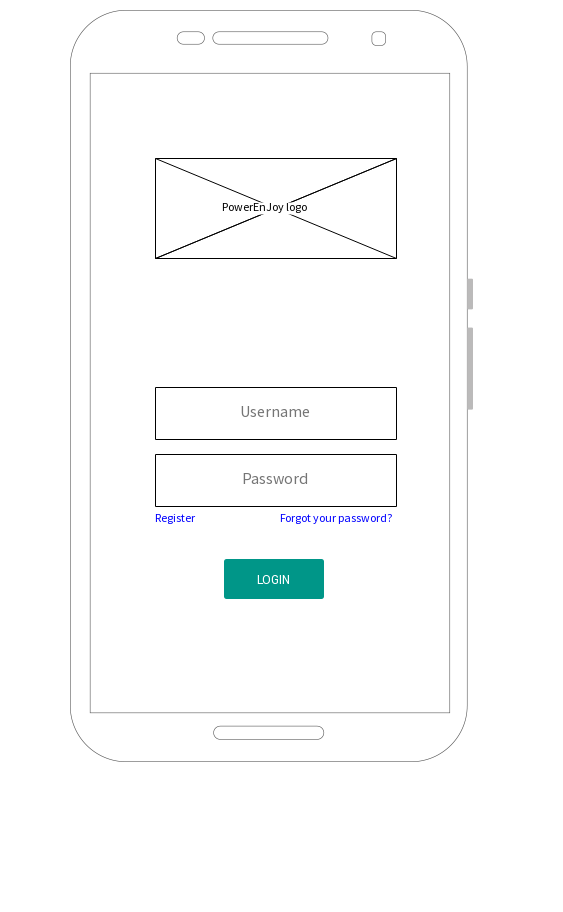
\includegraphics[width=\textwidth]{../UI/LoginScreen}
        \caption{Login Screen}
    \end{subfigure}
    ~
    \begin{subfigure}[b]{0.45\textwidth}
        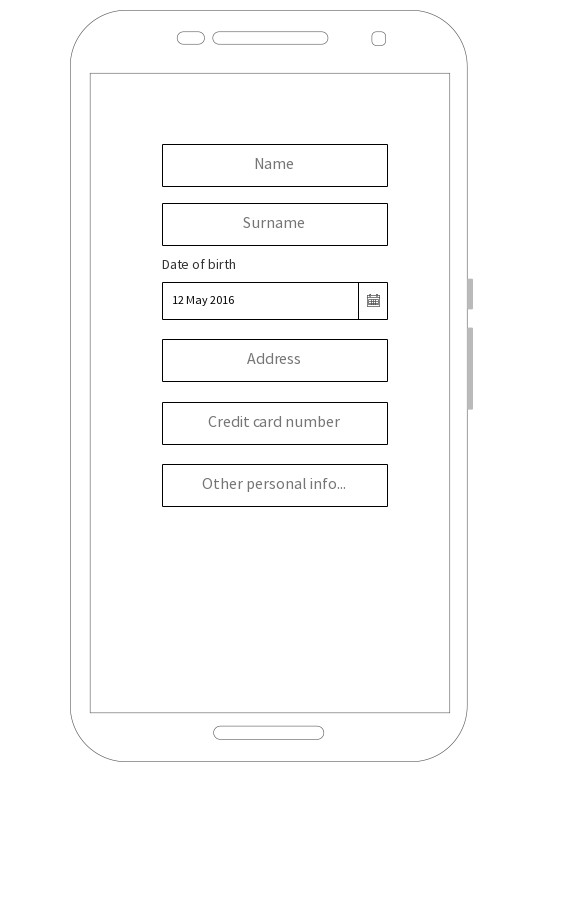
\includegraphics[width=\textwidth]{../UI/RegisterScreen}
        \caption{Register Screen}
    \end{subfigure}
\end{figure}
The Login and Register Screens are the only parts of the application that are accessible to Visitors. Registration can also be performed through the Company website, or Web Client. A User who logs in can access the Main Screen.\clearpage

\begin{figure}[h!]
    \centering
    \begin{subfigure}[b]{0.45\textwidth}
        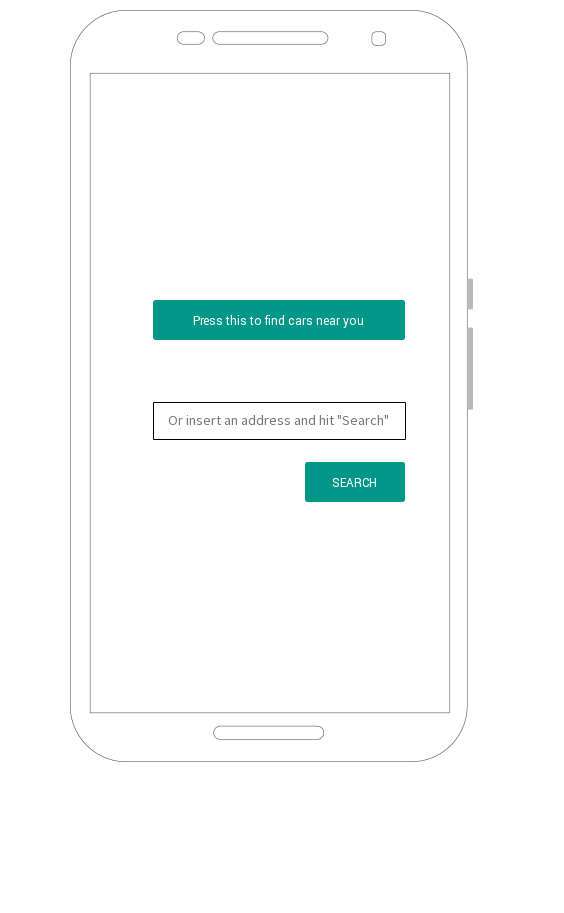
\includegraphics[width=\textwidth]{../UI/MainScreen}
        \caption{Main Screen}
    \end{subfigure}
    ~
    \begin{subfigure}[b]{0.45\textwidth}
        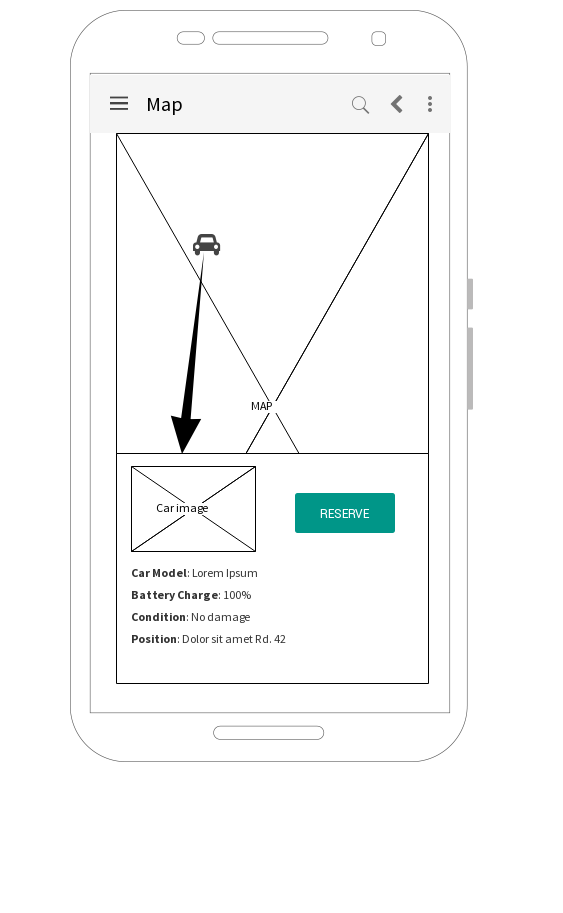
\includegraphics[width=\textwidth]{../UI/MapScreen}
        \caption{Map Screen}
    \end{subfigure}
\end{figure}
The Main Screen allows the User to view Cars near either their position or an address of their choice. From the Main Screen, the application shifts to the Map Screen, where all the eligible Cars are shown on a map, together with the position of the User. From this screen, the User can select one of the Cars shown and reserve it.\clearpage

\begin{figure}[h!]
    \centering
    \hspace{-2cm}
    \begin{subfigure}[b]{0.45\textwidth}
        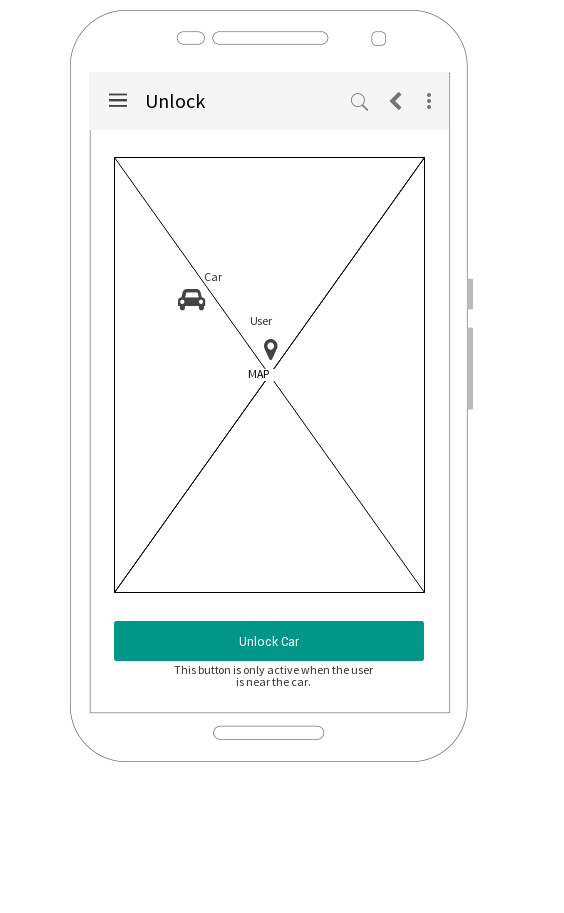
\includegraphics[width=\textwidth]{../UI/UnlockScreen}
        \caption{Unlock Screen}
    \end{subfigure}
    ~
    \begin{subfigure}[b]{0.64\textwidth}
        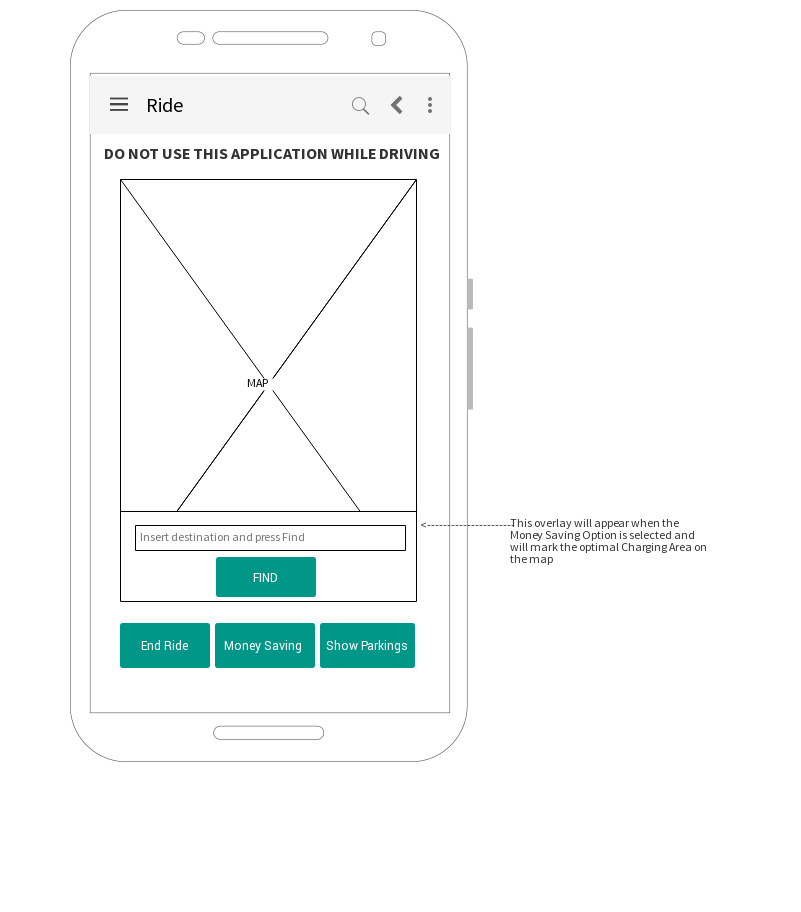
\includegraphics[width=\textwidth]{../UI/RideScreen}
        \caption{Ride Screen}
    \end{subfigure}
\end{figure}
After reserving a Car, the application will pass to the Unlock Screen, containing a map showing the User's position and that of the reserved Car. When the system detects that the User is close enough to the Car, the Unlock Car button becomes available.

While the Car is In Use, the application shifts to the Ride Screen, showing a map with the position of the User and allowing them to show on it the available Parking Areas or select the Money Saving Option to be notified of the optimal Charging Area where to park the Car. \clearpage

\begin{figure}[h!]
	\centering
	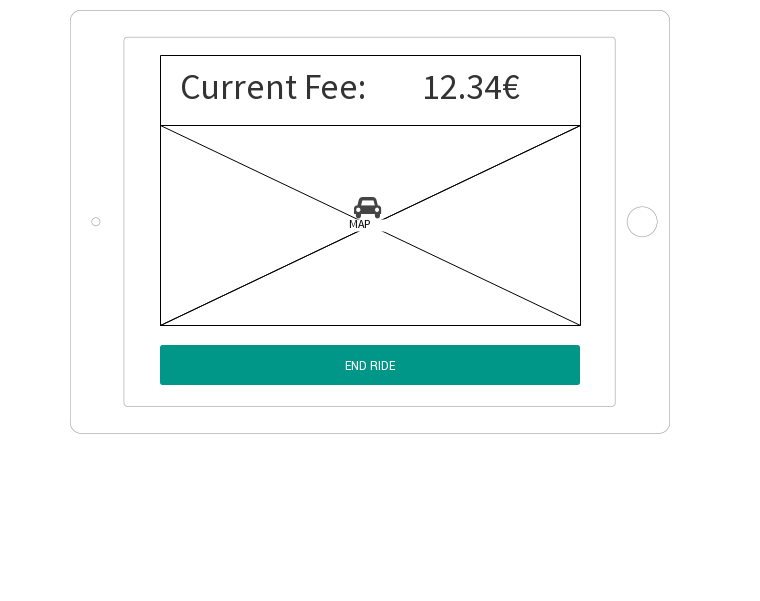
\includegraphics[width=0.9\textwidth]{../UI/CarScreen}
	\caption{Car Screen}
\end{figure}

The Car will have an internal computer showing a map of the area, the current Fee (not including any discount the User might be eligible for) and an "End Ride" button. Not pressing the button when leaving the Car will leave it In Use so that the User may leave the Car for a while if necessary (e.g. going to buy things without worrying that someone other might reserve the Car). However, it is worth noting that the Car is kept unlocked, and the User should be legally responsible for any improper use, theft or damage to the Car.

When the End Ride button is pressed, the Car will check to be parked in a Parking Area, then communicate all relevant data to the server.

\clearpage
\section{Requirements Traceability}
We need the Component Diagram for that.
\clearpage
\section{Hours of work}

\end{document}